\chapter{Especificação de Requisitos}
\label{sec:requisitos}

O processo de especificação de requisitos é crucial para o desenvolvimento de um projeto de \textit{software}, devendo dar atenção tanto aos requisitos funcionais como aos requisitos não funcionais.

Este capítulo apresenta os requisitos que foram identificados e analisados para a plataforma e define um conjunto de diretrizes que devem ser seguidas durante o desenvolvimento do projeto. Estes requisitos foram definidos e identificados com base em reuniões com o os responsáveis pelo projeto, necessidades que vão ao encontro do produto e na análise de soluções, atualmente no mercado, que partilham funcionalidades semelhantes com a plataforma que vai ser desenvolvida

Este capítulo divide-se em 3 secções. A secção \ref{requisitos:tiposutilizadores} identifica as principais partes envolventes no projeto (i. e. utilizadores e utilizadores finais). A secção \ref{rnf} e \ref{rf} descreve, detalhadamente, os requisitos não funcionais e funcionais, respectivamente. Por fim temos a secção \ref{prototipagem} que apresenta uma prototipagem de baixo nível, que com auxílio de breves descrições representa o fluxo da plataforma.


\section{Tipos de Utilizadores}
\label{requisitos:tiposutilizadores}

O objectivo desta secção é identificar, não necessariamente um problema, mas sim, através de uma estratégia de inbound marketing, uma forma de melhorar a experiência dos utilizadores proporcionando-lhes conteúdo que eles valorizam. Para melhor entender as necessidades do software é necessário fazer um estudo e tentar identificar os tipos de utilizadores finais, os seus comportamentos e fluxos de trabalho.


\subsection{\textit{Stakeholders}}

As principais partes envolventes neste projeto são, o proprietário do produto, os utilizadores principais e os utilizadores secundários. Como resultado os tipos de utilizadores serão baseados num público considerado  ideal, especulações e dados reais.


\subsection{Proprietário do produto}

O proprietário do produto é o Sr. Pedro Girão, \acrshort{ceo} na 10.digital. O aluno irá fazer o levantamento dos requisitos para o projeto que serão validados pelo proprietário do produto.

\subsection{Utilizadores primários}

A plataforma 10.quest tem dois tipos de utilizadores primários. Os primeiros são os utilizadores que irão utilizar o \textit{backoffice} da plataforma que fornece uma série de funcionalidades para criar campanhas com o conteúdo que lhes é fornecido, filtrar e segmentar os dados recolhidos e conseguir criar perfis de utilizador. O segundo tipo de utilizadores primários são os utilizadores finais. Os utilizadores finais irão participar nas campanhas (i. e. formações, questionários e/ou concursos) criadas pelo utilizador do \textit{backoffice}.


\subsection{Utilizadores secundários}

Apesar de não serem utilizadores diretos, todo o suporte e manutenção fornecida pela 10.digital, faz com que as pessoas responsáveis sejam \textit{stakeholders}, considerando o impacto que pode ter no seu fluxo de trabalho e produtividade geral no seu departamento. 
Outras entidades envolventes serão os responsáveis pela criação dos conteúdos que serão utilizados na plataforma.


\section{Requisitos Não Funcionais}
\label{rnf}

Nesta secção serão listados os requisitos não funcionais. Estes atributos dizem respeito aos atributos de qualidade da plataforma e foram identificados durante a fase de planeamento, adequando-se às necessidades do cliente e à natureza do produto. A lista de requisitos não funcionais é a seguinte:

\begin{itemize}
	\item \textbf{RNF01 - Segurança}
	\subitem - Um utilizador tem de estar autenticado para conseguir utilizar as funcionalidades da plataforma e apenas tem acesso a dados associados à sua conta. A comunicação com o \acrshort{tcg} será controlada com \textit{tokens}, para se controlar o acesso aos dados (i. e. um utilizador, autenticado ou não, não consegue efectuar pedidos de dados de outros utilizadores).
	\subitem - Medição: Testes de segurança.
	
	\item \textbf{RNF02 - Usabilidade} 
	\subitem - Um utilizador novo deve conseguir utilizar a plataforma (i. e. dominar todas as funcionalidades principais) em menos de 1 hora.
	\subitem - Medição: Testes de usabilidade
	
	\item \textbf{RNF03 - Disponibilidade}
	\subitem Sem contar com falhas de rede, o sistema deve garantir uma disponibilidade  igual ou superior a 98\%.
	\subitem - Medição: Arquitetura de Software.
	
	\item \textbf{RNF04 - Desempenho}
	\subitem - A plataforma não deve demorar mais do que 4 segundos a executar um pedido efectuado pelo utilizador sendo que nos primeiros 2 segundos já deve mostrar alguma informação.
	\subitem - Medição: Testes de stress.
	
	\item \textbf{RNF05 - Robustez}
	\subitem - O sistema deve ser tolerante a falhas, erros e outras condições anormais. Eventos como falhas em pedidos à base de dados ou ao \acrshort{tcg}, \textit{inputs} inválidos, falhas de rede, dados inválidos etc., devem ser tratados de forma a não ter impacto negativo na plataforma.
	\subitem - Medição: Testes de \textit{White Box} e \textit{Black Box}.
\end{itemize}


\section{Requisitos Funcionais}
\label{rf}

Nesta secção serão analisados e detalhados todos os requisitos funcionais da plataforma.

Numa primeira fase serão descritos os vários diagramas que representam todos os requisitos funcionais do sistema, seguindo a legenda da Figura \ref{fig:rf-legenda}. Estes diagramas têm como principal objectivo contextualizar e dar uma visão global de todos os requisitos do sistema. É ainda de notar que para diminuir a complexidade e facilitar a compreensão dos diagramas, os requisitos de menor dimensão que não justificam a criação de um caso de uso estão nos diagramas para complementar alguns casos de uso (i. e. requisitos de maior relevância) contudo estão identificados com uma cor diferente. Desta forma é possível focarmo-nos apenas nos requisitos de maior relevância.

\begin{figure}[ht!]
	\begin{center}
		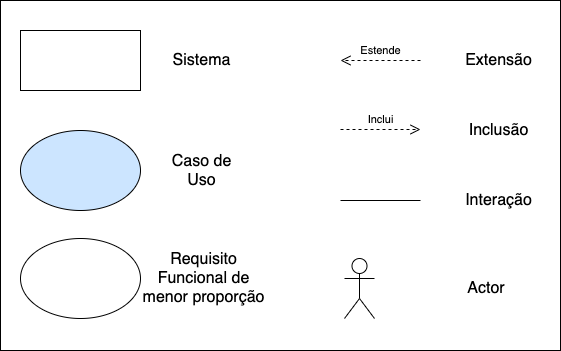
\includegraphics[width=0.7\textwidth]{img/rf/legenda}
		\caption{Legenda dos diagramas}
		\label{fig:rf-legenda}
	\end{center}
\end{figure}

Numa segunda fase serão analisados os graus de prioridade de cada requisito, consoante a sua importância para o projeto e por fim será feita uma descrição detalhada (i. e. especificação do requisito) de cada requisito através de casos de uso. É de notar que parte do grande trabalho da análise do grau de prioridade dos requisitos será imediato devido às decisões por parte do cliente.

Desta forma será claro para o leitor, mas em especial para a equipa de desenvolvimento, o comportamento que o sistema terá de cumprir. Os casos de uso serão detalhados consoante a seguinte estrutura:

\begin{itemize}
	\item \textbf{ID:} ID do caso de uso.
	\item \textbf{Ator:} Responsável pela realização do caso de uso.
	\item \textbf{Prioridade:} Representa a prioridade do caso de uso baseada nas decisões do cliente, visão dos stakeholders e no funcionamento do sistema. As prioridades foram classificadas por:
	\begin{itemize}
		\item \textbf{\textit{Must Have}:} Como o próprio nome indica, os requisitos \textit{Must} são os requisitos com maior prioridade. \textit{"As a rule, product inception depends entirely on defining must-haves using such pointers as ‘required for launch’, ‘required for safety’, ‘required for validation’, ‘required to deliver a viable solution’, etc."}\cite{moscow}. Todos os requisitos categorizados como \textit{Must Have}, são de implementação obrigatória pela equipa de desenvolvimento, uma vez que, sem eles o projeto fica paralisado.\textit{ "Can we move forward with the project if this task is undone? – if \textbf{NO}, it’s \textbf{MUST}"}\cite{moscow}.
		\item \textbf{\textit{Should Have}:} Os requisitos \textit{Should} são requisitos que também têm uma elevada prioridade, ou por outras palavras, estão apenas um passo abaixo dos requisitos \textit{Must}.
		Não são requisitos considerados vitais contudo adicionam valor significativo.\textit{ "Will we move forward with the project if this task is done a bit later? – if \textbf{YES}, it’s \textbf{SHOULD}"}\cite{moscow}.
		\item \textbf{\textit{Could Have}:} Os requisitos \textit{Could} são requisitos com menos importancia e impacto que os anteriores. Pode-se dizer, por outras palavras, que são requisitos \textit{Nice to have} e tipicamente só são implementados se houver tempo para tal. \textit{ "Can we sacrifice this task till deadline? – if \textbf{YES}, it’s \textbf{COULD}"}\cite{moscow}.
		\item \textbf{\textit{Won't Have}:} Os requisitos \textit{Won't} são os requisitos com menor prioridade. Os requisitos categorizados com esta prioridade, tipicamente não são implementados no tempo estipulado para o projeto. Alguns requisitos são priorizados no futuro, outros nunca chegam a ser implementados. \textit{ "Can we back to it when things go better? – if \textbf{YES}, it’s \textbf{WON’T}"}\cite{moscow}.
	\end{itemize}
	\item \textbf{Descrição:} Uma breve contextualização do caso de uso.
	\item \textbf{Pré-condições:} Conjunto de condições necessárias para realizar o caso de uso.
	\item \textbf{Estímulo:} Casos de uso responsáveis pela ativação do caso de uso.
	\item \textbf{Fluxo Principal:} Descrição detalhada de todos os passos para a realização do casos de uso.
	\item \textbf{Fluxo de Excepção:} Descrição detalhada do comportamento do sistema quando o caso de uso não for realizado com sucesso.
	\item \textbf{Observações:} Observações adicionais, relevantes para o desfecho do caso de uso.
\end{itemize}

\newpage

\subsection{Diagrama de contexto}
\label{d:contexto}
\begin{figure}[ht!]
	\begin{center}
		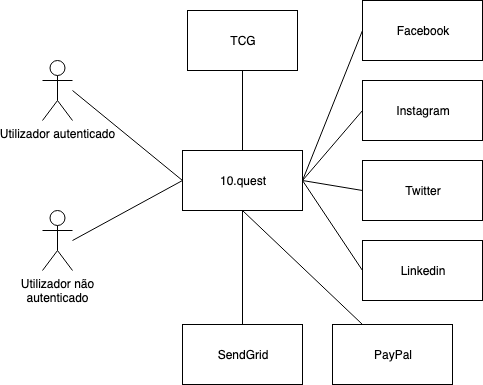
\includegraphics[width=0.6\textwidth]{img/rf/10quest}
		\caption{Diagrama de contexto}
		\label{fig:rf-10quest}
	\end{center}
\end{figure}

A 10.quest, tal como referido nos capítulos anteriores, é uma plataforma de inbound marketing que permite aos utilizadores criar campanhas e tratar a informação recolhida nas mesmas. 
Estas campanhas poderão ser partilhados nas redes sociais (i. e. utilizando a API do Facebook, Instagram e Twitter) através de \textit{landing pages}. Estas \textit{landing pages} terão um pequeno formulário que necessita das informações básicas ao utilizador final para que, automaticamente, as formações, questionários e concursos sejam enviados por mail para os inscritos, utilizando o sistema externo SendGrid.

Tal como referido no Capítulo \ref{sec:estado-arte}, o \acrshort{tcg} é um produto desenvolvido pela 10.digital e encontra-se atualmente no mercado. Algumas das funcionalidades fundamentais da plataforma a desenvolver já estão implementadas no \acrshort{tcg}  e por isso mesmo haverá uma integração com o mesmo para aproveitar todas estas funcionalidades necessárias.


\newpage

\subsection{Diagrama de alto nível}
\label{d:altonivel}
\begin{figure}[ht!]
	\begin{center}
		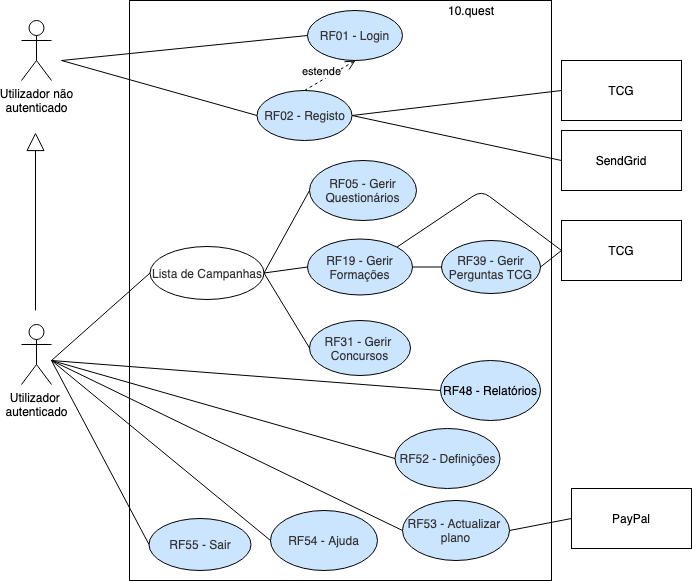
\includegraphics[width=0.8\textwidth]{img/rf/alto-nivel}
		\caption{Diagrama de Alto Nível}
		\label{fig:rf-alto-nivel}
	\end{center}
\end{figure}

Um utilizador para aceder a todas as funcionalidades da plataforma terá de primeiro realizar a autenticação (\textbf{RF01 - Login}). Caso ainda não tenha uma conta registada terá de o fazer. Assim que a conta for criada é enviada uma notificação para o email do utilizador, recorrendo ao sistema externo SendGrid. Por questões de segurança e confidencialidade dos dados, no acto do registo, a informação do utilizador será enviada e guardada na base de dados do \acrshort{tcg}, para que mais tarde todos os pedidos REST possam ser validados.

Depois de um utilizador se autenticar, será direcionado para a página inicial. A partir daqui o utilizador tem acesso à sua lista de campanhas (i. e. questionários, formações e concursos) podendo gerir as mesmas; aceder às definições, atualizar o plano da conta, utilizar o suporte da plataforma e terminar sessão.
Ainda na página inicial da plataforma, onde se encontram listados todos os tipos de campanhas do utilizador da plataforma, será exibido o estado de cada campanha e data de termino, se for o caso, para ajudar o utilizador a perceber de forma rápida o estado das mesmas.

\newpage

\subsection{Diagrama Registo}
\label{d:registo}
\begin{figure}[ht!]
	\begin{center}
		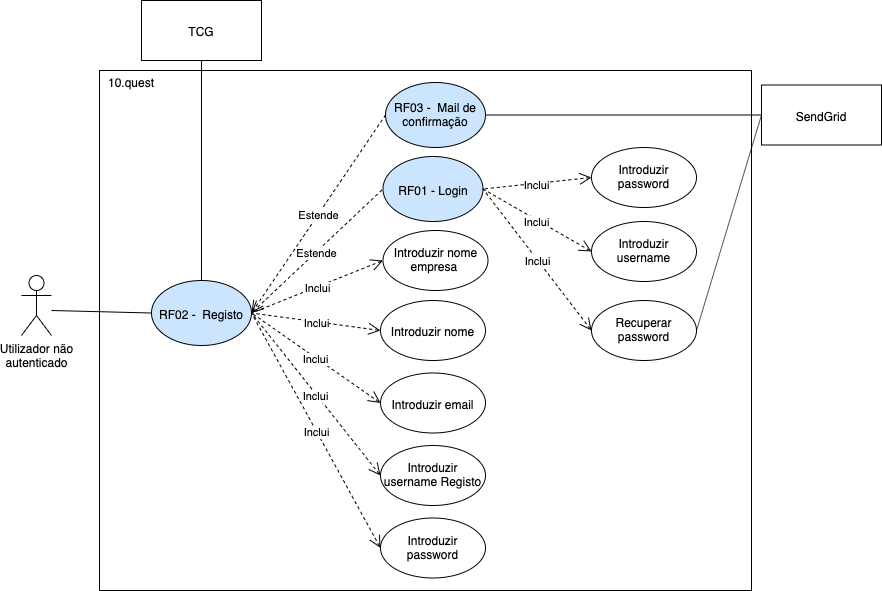
\includegraphics[width=1\textwidth]{img/rf/registo}
		\caption{Diagrama Gerir Concursos}
		\label{fig:rf-registo}
	\end{center}
\end{figure}

Para se efetuar um registo é necessário introduzir o nome da empresa, nome do utilizador, email, \textit{username} e \textit{password}. De seguida é enviado um mail de validação para o email associado à conta.

Depois de validada a conta do utilizador, este consegue efetuar o \textit{login} na plataforma.



\newpage

\subsection{Diagrama Gerir Perguntas de Formação}
\label{d:perguntastcg}
\begin{figure}[ht!]
	\begin{center}
		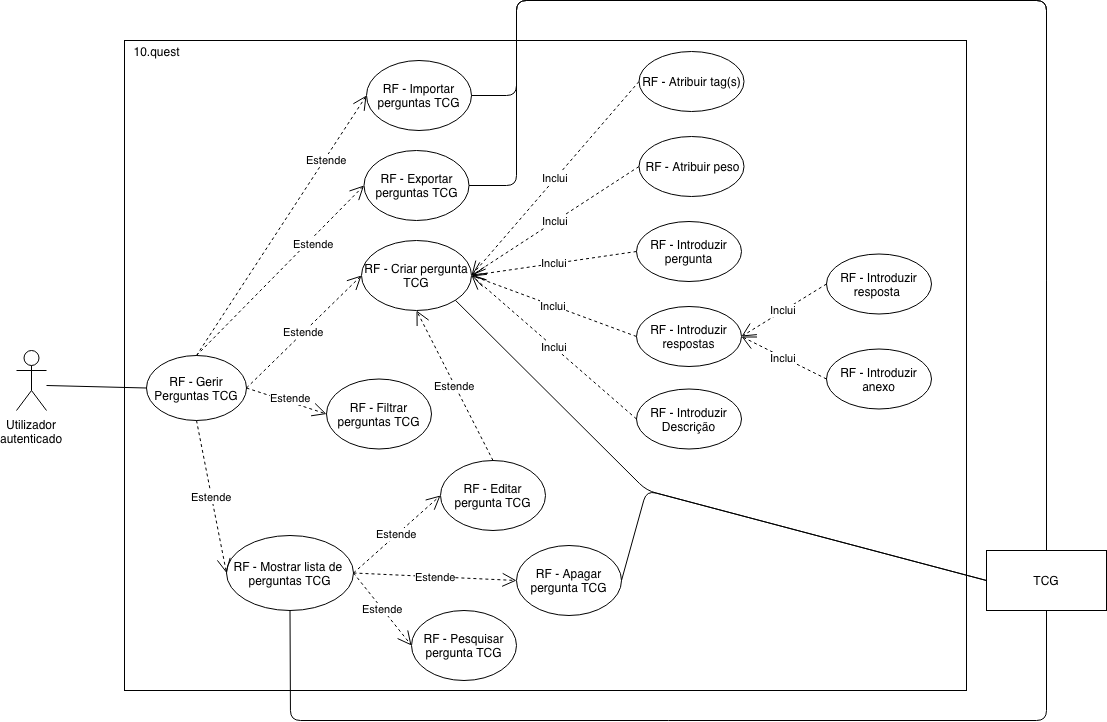
\includegraphics[width=1\textwidth]{img/rf/gerir-perguntas-tcg}
		\caption{Diagrama Gerir Perguntas de Formação}
		\label{fig:rf-gerir-perguntas-tcg}
	\end{center}
\end{figure}

No \acrshort{tcg}, tal como referido no anexo \ref{sec:TCG}, a criação de questões é isolada da criação de formações. Esta abordagem traz uma série de vantagens, referidas no Capítulo \ref{sec:TCG}, e neste sentido, este será o modelo seguido. Dito isto, é necessário primeiro criar questões para que se possa ter conteúdos para as formações. 

É ainda de notar que por uma questão de terminologia, na plataforma a desenvolver, as Perguntas de Formação são equivalentes às questões no \acrshort{tcg}, pelo simples facto de não se confundir com elementos relacionados com os questionários de personalidade.

Na gestão de perguntas de formação, um utilizador consegue listar todas as perguntas (\textbf{RF45 - Mostrar lista de perguntas de formação}) associadas à sua conta (i. e. criadas por ele) e pode também criar uma nova pergunta (\textbf{RF42 - Criar pergunta de formação}). Para editar uma pergunta (\textbf{RF46 - Editar pergunta de formação}) é necessário aceder à mesma através da lista, sendo que é possível organizar e pesquisar por nome ou tag, e é ainda possível selecionar multiplas perguntas de formação para eleminar (\textbf{RF47 - Apagar pergunta de formação}). As perguntas podem também ser importadas e exportadas através de uma \textit{spreadsheet}.

Para um criar uma pergunta (\textbf{RF42}), o utilizador precisa de atribuir uma tag, nova ou existente, introduzir a pergunta e as respostas. Cada pergunta tem que ter obrigatoriamente uma resposta certa e pelo menos uma resposta errada, sendo estas compostas pela resposta e um anexo opcional que pode ser uma imagem ou vídeo.



\newpage

\subsection{Diagrama Gerir Formações}
\label{d:formacoes}
\begin{figure}[ht!]
	\begin{center}
		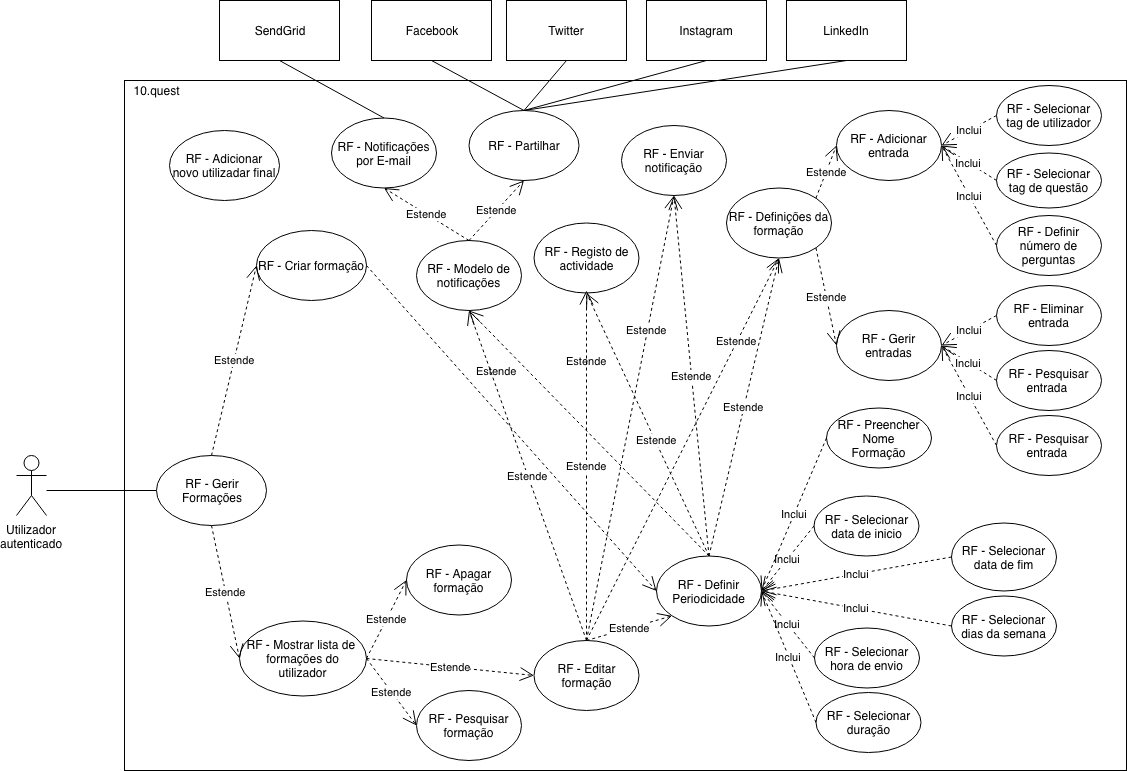
\includegraphics[width=1\textwidth]{img/rf/gerir-formacoes}
		\caption{Diagrama Gerir Formações}
		\label{fig:rf-gerir-formacoes}
	\end{center}
\end{figure}

Quase todas as funcionalidades necessárias para a gestão de formações já estão implementadas no \acrshort{tcg}. Neste sentido terá que ser apenas garantido um conjunto de requisitos que permita ao utilizador reuniar as condições necessárias para utilizar as capacidades do TCG através de pedidos REST. Isto implica ter uma interface completa no lado do 10.quest e selecionar quais os dados a guardar no 10.quest e no \acrshort{tcg}, respetivamente, garantindo sempre a sincronização dos dados.

Na gestão de formações um utilizador consegue listar todas as formações associadas à sua conta (\textbf{RF27 - Mostrar lista de formações do utilizador}) e pode também criar uma nova formação (\textbf{RF20 - Criar formação}).
Para criar uma formação (\textbf{RF20}) o utilizador terá, numa primeira instância, de atribuir um nome e definir a periodicidade (i. e. preencher a hora de envio, dias da semana,  duração e validade) (\textbf{RF21 - Definir periodicidade}). 
Numa segunda fase, o utilizador, através do requisito \textbf{RF - Definições da formação} consegue adicionar e gerir entradas de perguntas de formações(\textbf{RF25 - Adicionar entrada de perguntas} e \textbf{RF26 - Gerir entradas de perguntas}, respectivamente). É através destas entradas que o utilizador da plataforma associa perguntas à formação. Para adicionar uma entrada (\textbf{RF25 - Adicionar entrada de perguntas} ) o utilizador da plataforma seleciona as perguntas que deseja através de tags (i.e. as perguntas com as tags respectivas são associadas) e o número de perguntas que o utiliador final irá receber, com esse mesmo perfil de tags.

Por fim o utilizador pode partilhar a formação (\textbf{RF56 - Partilhar}). As inscrições numa formação serão feitas através de uma \textit{landing page} que pode ser personalizada no requisito \textbf{RF08 - Landing Page} e enviadas para o email introduzido no mini formulário da \textit{landing page}. Este mail com o link para a formação, pode ser personalizado no requisito \textbf{RF09 - Notificações por E-mail}. 

É de notar que, através do requisito \textbf{RF29 - Adicionar novo utilizador final TCG}, sempre que um utilizador final se inscreve numa formação através da \textit{landing page}, o sistema, de forma automática, envia os dados para \acrshort{tcg} para que este utilizador possa começar a receber a formação por email. Outro requisito da responsabilidade do sistema é o \textbf{RF30 - Notificar utilizadores finais TCG}, que respeitando a periodicidade definida na criação do formação, envia a formação para todos os inscritos.



\subsection{Diagrama Gerir Questionários}
\label{d:quests}
\begin{figure}[ht!]
	\begin{center}
		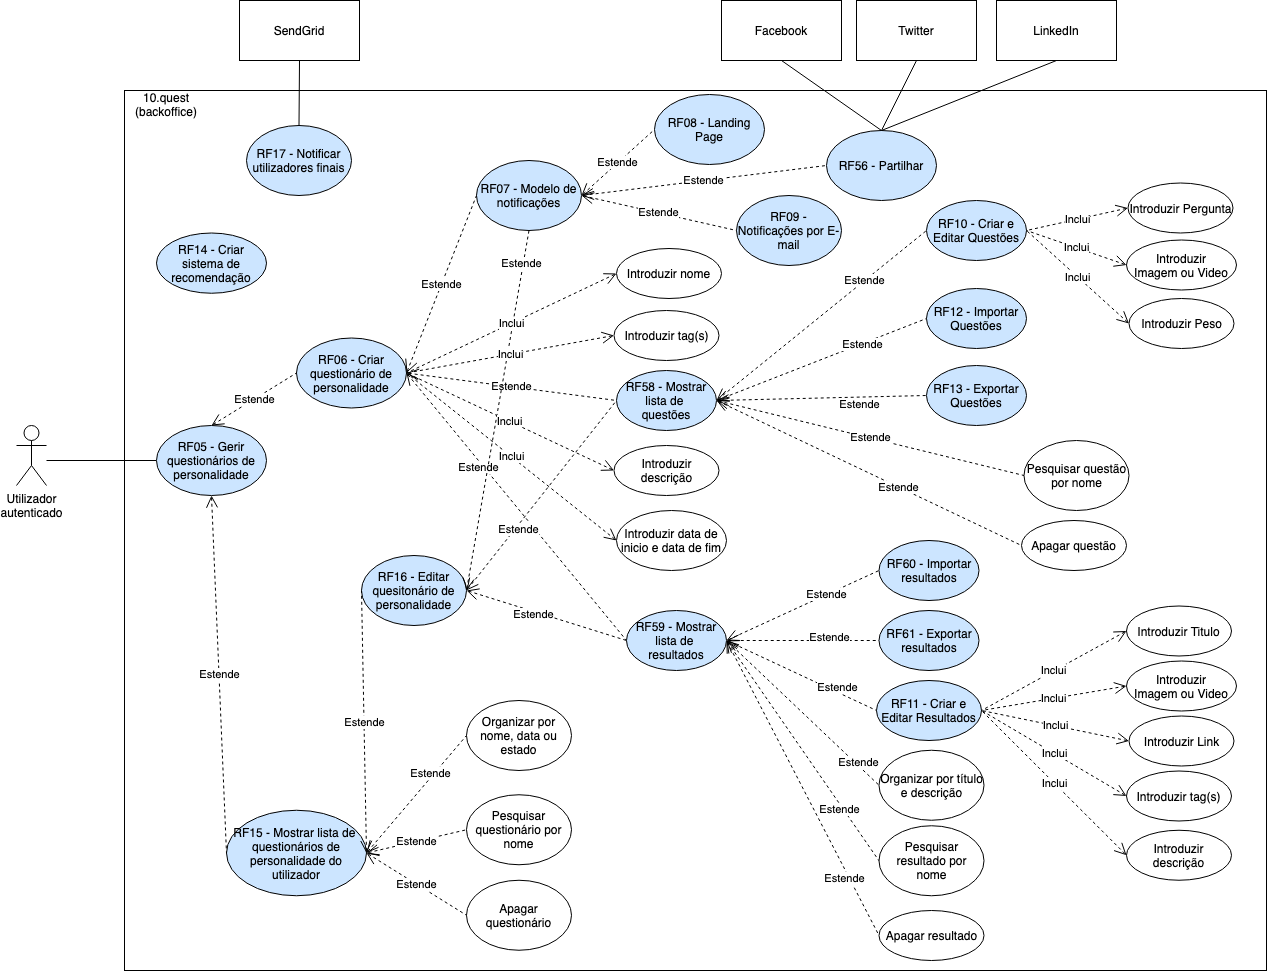
\includegraphics[width=1\textwidth]{img/rf/gerir-quest}
		\caption{Diagrama Gerir Questionários}
		\label{fig:rf-gerir-quest}
	\end{center}
\end{figure}

Na gestão de questionários, à semelhança da gestão de formações, é feita uma listagem dos questionários (\textbf{RF15 - Mostrar lista de questionários do utilizador}) e o utilizador tem a capacidade de criar (\textbf{RF06 - Criar questionário}), eliminar, editar (\textbf{RF16 - Editar questionário}) e pesquisar questionários.

Na criação de um novo questionário (\textbf{RF06}), um utilizador, numa primeira fase terá de criar um conjunto de questões (\textbf{RF10 - Criar questões}) e gerar um série de resultados (\textbf{RF11 - Criar resultados}). Cada resultado terá de ter obrigatoriamente uma \textit{tag} associada e um título e caso o utilizador deseje uma imagem e/ou um link. As perguntas e resultados podem também ser importados e exportados numa \textit{spreadsheet}.

Depois de terminar a primeira fase, podendo a qualquer momento voltar a essa fase, o utilizador já tem recursos para começar a construir o questionário (i. e. o sistema de pontuação através do requisito \textbf{RF14 - Criar sistema de pontuação}). Numa primeira instância o utilizador terá de selecionar a pergunta pelo qual deseja começar o questionário.
De seguida cria uma ou mais respostas possíveis e para cada uma destas respostas é necessário indicar a pergunta que se segue, caso a respectiva resposta seja escolhida. Desta forma o utilizador consegue criar um fluxo de perguntas.
%De seguida cria uma ou mais respostas e para cada uma delas é necessário associar uma pergunta que na iteração seguinte sejam apresentadas e se possa repetir este processo para conseguir criar um fluxo de perguntas.
 Para cada pergunta é atribuído um peso e para cada resposta são associadas \textit{tags} de resultados. Desta forma numa dada pergunta, as \textit{tags} da resposta selecionada serão pontuadas. A qualquer momento o utilizador, em vez de associar uma pergunta a uma resposta, pode decidir, naquele estado (i. e. numa resposta em específico), terminar o questionário e apresentar o resultado ao utilizador final.

Através do requisito \textbf{RF18 - Adicionar novo utilizador final}, sempre que um utilizador final se inscreve num questionário através da \textit{landing page}, o sistema, de forma automática, guarda essa informação e recorrendo ao requisito \textbf{RF17 - Notificar utilizadores finais}, envia o questionário para o utilizador final.


\subsection{Diagrama Gerir Concursos}
\label{d:concursos}
\begin{figure}[ht!]
	\begin{center}
		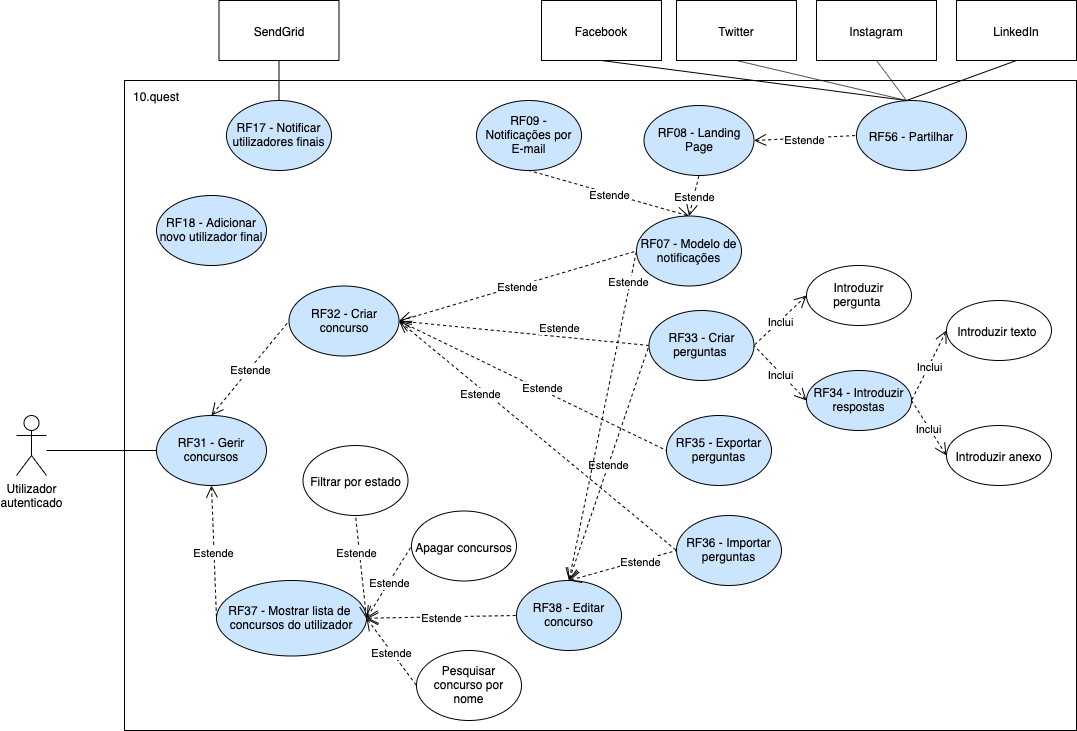
\includegraphics[width=1\textwidth]{img/rf/gerir-concurso}
		\caption{Diagrama Gerir Concursos}
		\label{fig:rf-gerir-concursos}
	\end{center}
\end{figure}


Na gestão de concursos, à semelhança da gestão de formações e questionários, é feita uma listagem dos concursos (\textbf{RF37 - Mostrar lista de concursos do utilizador}) e o utilizador tem a capacidade de criar (\textbf{RF32 - Criar concurso}), eliminar, editar (\textbf{RF38 - Editar concurso}) e pesquisar questionários.

Na criação de um concurso (\textbf{RF32}) o utilizador terá de criar perguntas (\textbf{RF33 - Criar perguntas}). Para cada pergunta o utilizador terá de introduzir pelo menos duas respostas (\textbf{RF34 - Introduzir respostas}) e caso o desejo pode adicionar um anexo no formato de imagem. As perguntas e respostas podem também ser importados e exportados numa \textit{spreadsheet} (\textbf{RF36 - Importar perguntas} e \textbf{RF35 - Exportar perguntas}, respectivamente).

É importante referenciar que à semelhança da gestão de formações e questionários, é possível editar os conteúdos (i. e. perguntas, questões, \textit{landing pages}, email etc) contudo, assim que um concurso é publicado e passa a estar no estado \textit{online}, as perguntas deixam de poder ser editáveis. 

Os concursos, tal como os questionários têm sempre um estado que pode variar entre:
\begin{itemize}
	\item Rascunho - Utilizador não deu o lançamento do concurso como concluído.
	\item Aberto - Utilizador deu o lançamento do concurso como concluído.
	\item \textit{Online} - Utilizador gerou a \textit{landing page} para partilhar o concurso.
	\item Fechado - Concurso chegou à data de fim.
\end{itemize}


\subsection{Diagrama Ajuda}
\label{d:ajuda}
\begin{figure}[ht!]
	\begin{center}
		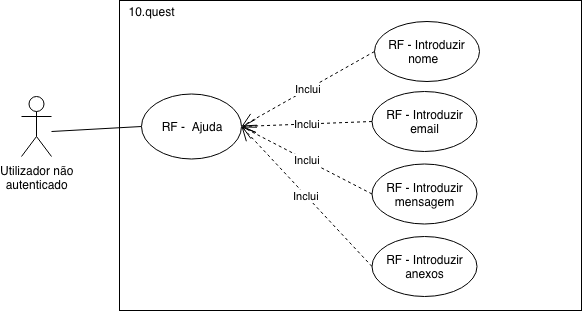
\includegraphics[width=1\textwidth]{img/rf/ajuda}
		\caption{Diagrama Ajuda}
		\label{fig:rf-ajuda}
	\end{center}
\end{figure}


O utilizador poderá, se assim o pretender, utilizar o suporte da plataforma. Em caso de dúvida ou esclarecimentos, enviar uma mensagem direta para a 10.digital. 

Para enviar uma mensagem é necessário introduzir o nome, email, mensagem e, caso o utilizador deseje, um ou mais anexos.

\newpage

\subsection{Diagrama Relatórios}
\label{d:relatorios}

\begin{figure}[ht!]
	\begin{center}
		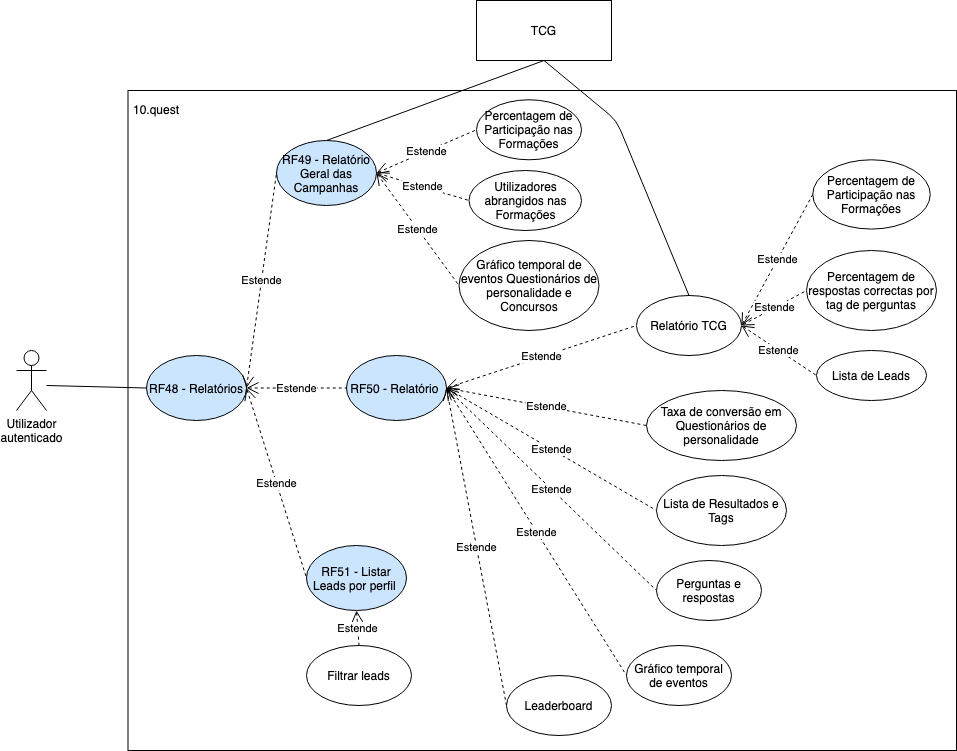
\includegraphics[width=1\textwidth]{img/rf/relatorio}
		\caption{Diagrama Relatórios}
		\label{fig:rf-relatorios}
	\end{center}
\end{figure}

Assim que uma formação, questionário ou concurso terminar, ou a qualquer momento, um utilizador pode gerar o relatório de dados. A secção de dados da plataforma mostra os resultados gerais sobre as formações, questionários e concursos (\textbf{RF49 - Relatório geral}). 

O utilizador pode gerar um relatório (\textbf{RF50 - Relatório}) para um questionário onde será exposto o resultados do mesmo. Será mostrado um gráfico de conversão de tipos de utilizadores finais e uma secção onde se pode calcular a taxa de conversão. Serão também mostrados os resultados do questionário e as respostas por pergunta. Pode ser ainda visto, no final, um gráfico temporal de eventos.

Para os relatórios de concursos será exposta uma tabela com as classificações de cada participante e para os relatórios de uma formação será feito um pedido ao TCG para retornar o relatório relativo à formação selecionada.

Por fim, na secção de dados (i. e. relatórios) o utilizador pode navegar na lista de leads (\textbf{RF51 - Listar Leads por perfil}) que vão participando nas suas formações, questionários e concursos. Esta lista terá todos os utilizadores finais listados que são considerados leads e é possível filtrar os mesmos por tags (i. e. criar um perfil de utilizador). Para cada utilizador serão apresentados os dados pessoais que eles vão fornecendo ao longo da jornada (e. g. nome, email etc...)




\section{Mockups}
\label{prototipagem}

A criação de mockups/protótipos de baixa fidelidade, teve como principal objetivo representar a plataforma (i. e. todos os requisitos funcionais) de forma estática. Esta secção foi importante para conseguir visualizar a plataforma como um todo, facilitando a implementação, e também teve um papel importante na verificação dos requisitos levantados, satisfazendo todos os casos de uso descritos no Anexo \ref{a:cu}. Todos os mockups realizados encontram-se descritos no Anexo \ref{a:prototipos}.


%-------------------------------------------------------------------------------------------------
\blankpage
%-------------------------------------------------------------------------------------------------

\glsresetall